
\section{CNN: tricks for visualization (Alfredo Canziani)}
% Authors: Pedro Manuel Herrero Vidal, Doruk Kilitcioglu
% Lecture date: 2/27/2019

We take the data simulated in the 04-spiral\_classification notebook (\href{https://github.com/Atcold/pytorch-Deep-Learning-Minicourse/blob/master/04-spiral\_classification.ipynb} {"Spiral Classification"}), 
consisting of 3,000 samples of dimension 2 (Fig. ~\ref{fig:NonLinearlySeparableParametricCurves2}). 
The data is generated from the following expression:

\[
X_c(t) = t
\begin{bmatrix}
    \sin{\frac{2\pi}{C} (2t+c+1) + \mathcal{N} (0, \sigma^2)} \\
    \cos{\frac{2\pi}{C} (2t+c+1) + \mathcal{N} (0, \sigma^2)}
\end{bmatrix}
\]
%\noindent
where $0 \leq t \leq 1$ and classes $c=1, ..., C$.


\begin{figure}[ht]
\centering
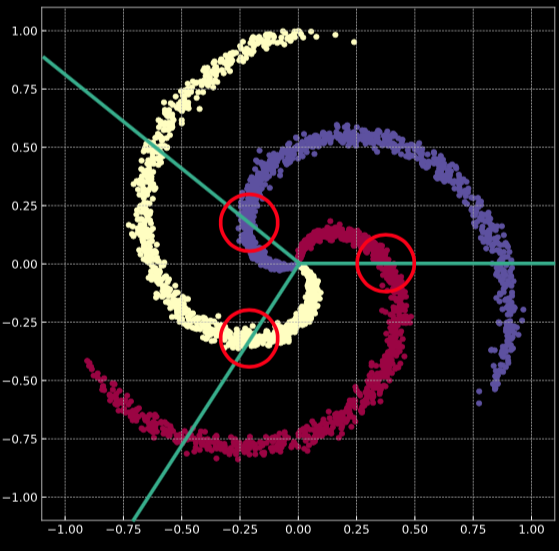
\includegraphics[width=0.5\textwidth]{lectures/04-a/images/NonLinearlySeparableParametricCurves.png}
\caption{3 non linearly separable curves consisting in 3,000 samples from $X \in {{\rm I\!R}}^2$.}
\label{fig:NonLinearlySeparableParametricCurves2}
\end{figure}

\noindent
To classify the data into the three categories, we are going to use a three layer net with: 
\begin{itemize}
\item[(1)] 2 input units (dimensionality of the data).
\item[(2)] A 100-units hidden layer (used to increase the space and extract features).
\item[(3)] Followed by a ReLU activation function that connects to a two-units layer (here is the trick for visualization!) 
\item[(4)] And then a linear transformation (with no non-linearity in between) to a 3-unit output layer with softmax activation function for classification 
(Fig. ~\ref{fig:ArchitectureForClassificationAndVisualizationInTheInputSpace}). 
Having a 2-unit layer (same as input layer) right before the output layer allows to visualize the transformations 
that the original space went throw to solve the classification task. 
The last linear transformation involves the multiplication of $A^{(3)}$ and $W^{(2)}$, 
where the different rows of $W^{(2)}$ are the 2D vectors that will point at the different classes in the 2D space. 
In this representation, the different classes are linearly separable.
\end{itemize}

\begin{figure}[!h]
\centering
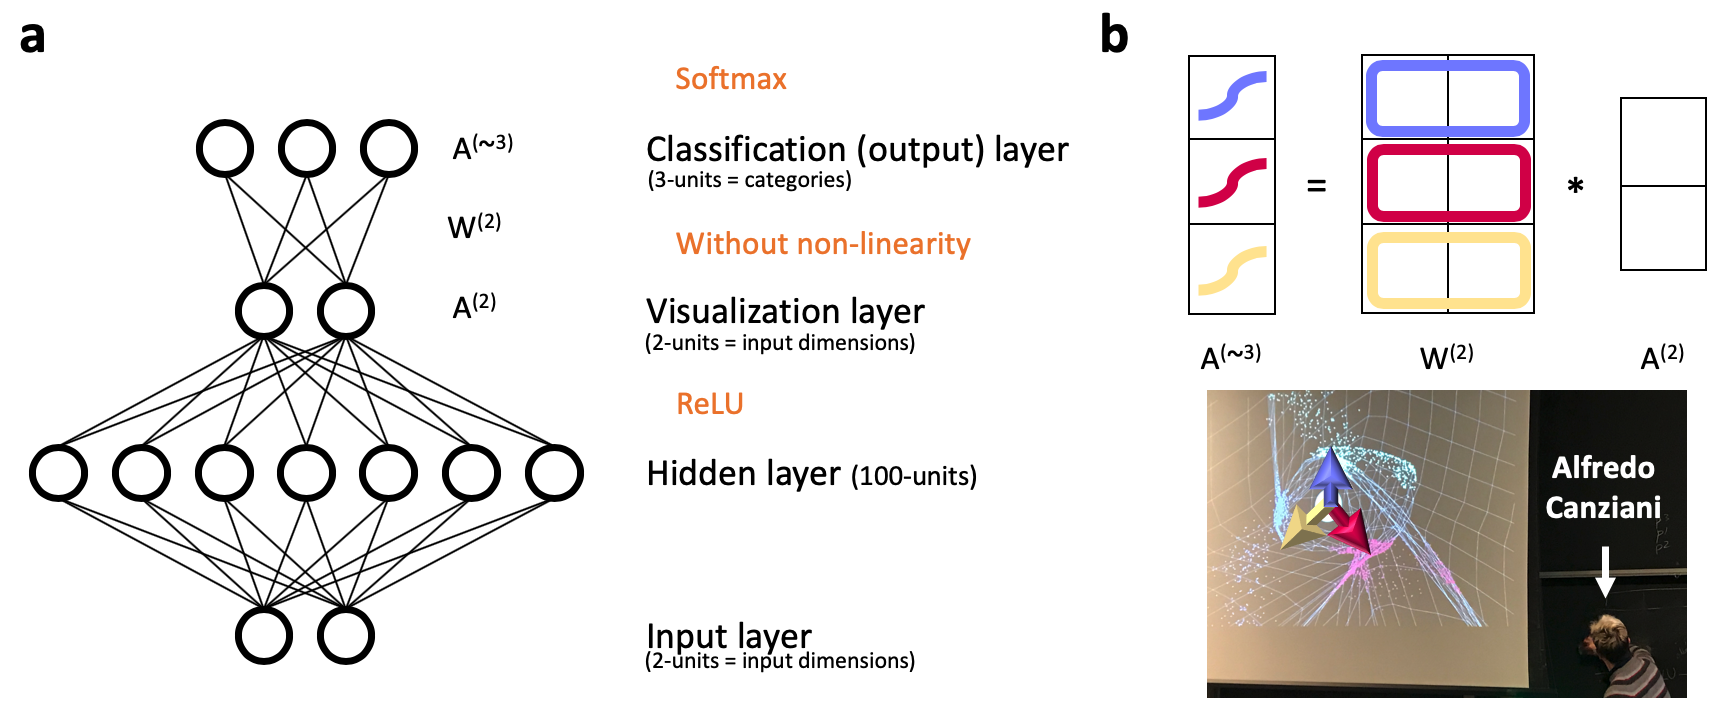
\includegraphics[width=170mm]{lectures/04-a/images/ArchitectureForClassificationAndVisualizationInTheInputSpace.png}
\caption{Neural network architecture for classification and visualization in the input space. (a) Architecture of the neural network, which takes 2D inputs and visualizes in the same dimensional space before classification. (b) Linear transformation that takes $A^{(2)}$ and returns $A^{(3)}$ via multiplication with $W^{(2)}$. Rectangular color boxes in $W^{(2)}$ represent the three 2D vectors that will define each class. Calculation of $A^{(3)}$ is followed by a softmax activation function for classification. In the bottom half of (b), the transformed data after and the population vectors (plot credit: Alfredo Canziani).}
\label{fig:ArchitectureForClassificationAndVisualizationInTheInputSpace}
\end{figure}

\noindent
We can linearly interpolate between the two data representations, before and 
after being feed into the network, in the 2D space by:

\[
(1-\alpha)(x^{(1)}) + \alpha \phi (x^{(i)}) ~~\text{ where } 0 \leq \alpha \leq 1
\]

